\documentclass[12pt, a4paper, oneside]{ctexart}
\usepackage{amsmath, amsthm, amssymb, bm, color, graphicx, geometry, hyperref, mathrsfs,extarrows, braket}

\linespread{1.5}
\geometry{left=2.54cm,right=2.54cm,top=3.18cm,bottom=3.18cm}
\newenvironment{problem}{\par\noindent\textbf{题目. }}{\bigskip\par}
\newenvironment{solution}{\par\noindent\textbf{解答. }}{\bigskip\par}
\newenvironment{note}{\par\noindent\textbf{注记. }}{\bigskip\par}

% 基本信息
\newcommand{\dt}{\today}
\newcommand{\sj}{离散数学}
\newcommand{\vt}{吴天阳 2204210460}

\begin{document}

\pagestyle{empty}
\vspace*{-20ex}
\centerline{\begin{tabular}{*3{c}}
    \parbox[t]{0.3\linewidth}{\begin{center}\textbf{日期}\\ \large \textcolor{blue}{\dt}\end{center}} 
    & \parbox[t]{0.3\linewidth}{\begin{center}\textbf{科目}\\ \large \textcolor{blue}{\sj}\end{center}}
    & \parbox[t]{0.3\linewidth}{\begin{center}\textbf{姓名,学号}\\ \large \textcolor{blue}{\vt}\end{center}} \\ \hline
\end{tabular}}
\vspace*{4ex}
\paragraph{习题八}
\paragraph{38.}\begin{solution}
    设图$G=(V,E)$满足题目条件,设$|V| = n$,由于$G$为一棵树,则$|E| = n-1$,由于
    \begin{equation*}
        \sum_{u\in V}\text{deg}(u) = 2|E| = 2(n-1)
    \end{equation*}
    则有
    \begin{equation*}
        \begin{cases}
            2(n-1) = \sum\limits_{u\in V}\text{deg}(u) = n_1+2n_2+3n_3+\cdots+kn_k\\
            n = n_1+n_2+\cdots+n_k
        \end{cases}
    \end{equation*}
    解得
    \begin{equation*}
        n_1 = n_3+2n_4+\cdots+(k-2)n_k+2=2+\sum_{i=3}^k(i-2)n_i
    \end{equation*}
\end{solution}
\paragraph{42.}\begin{solution}
    如图:

    \centerline{
        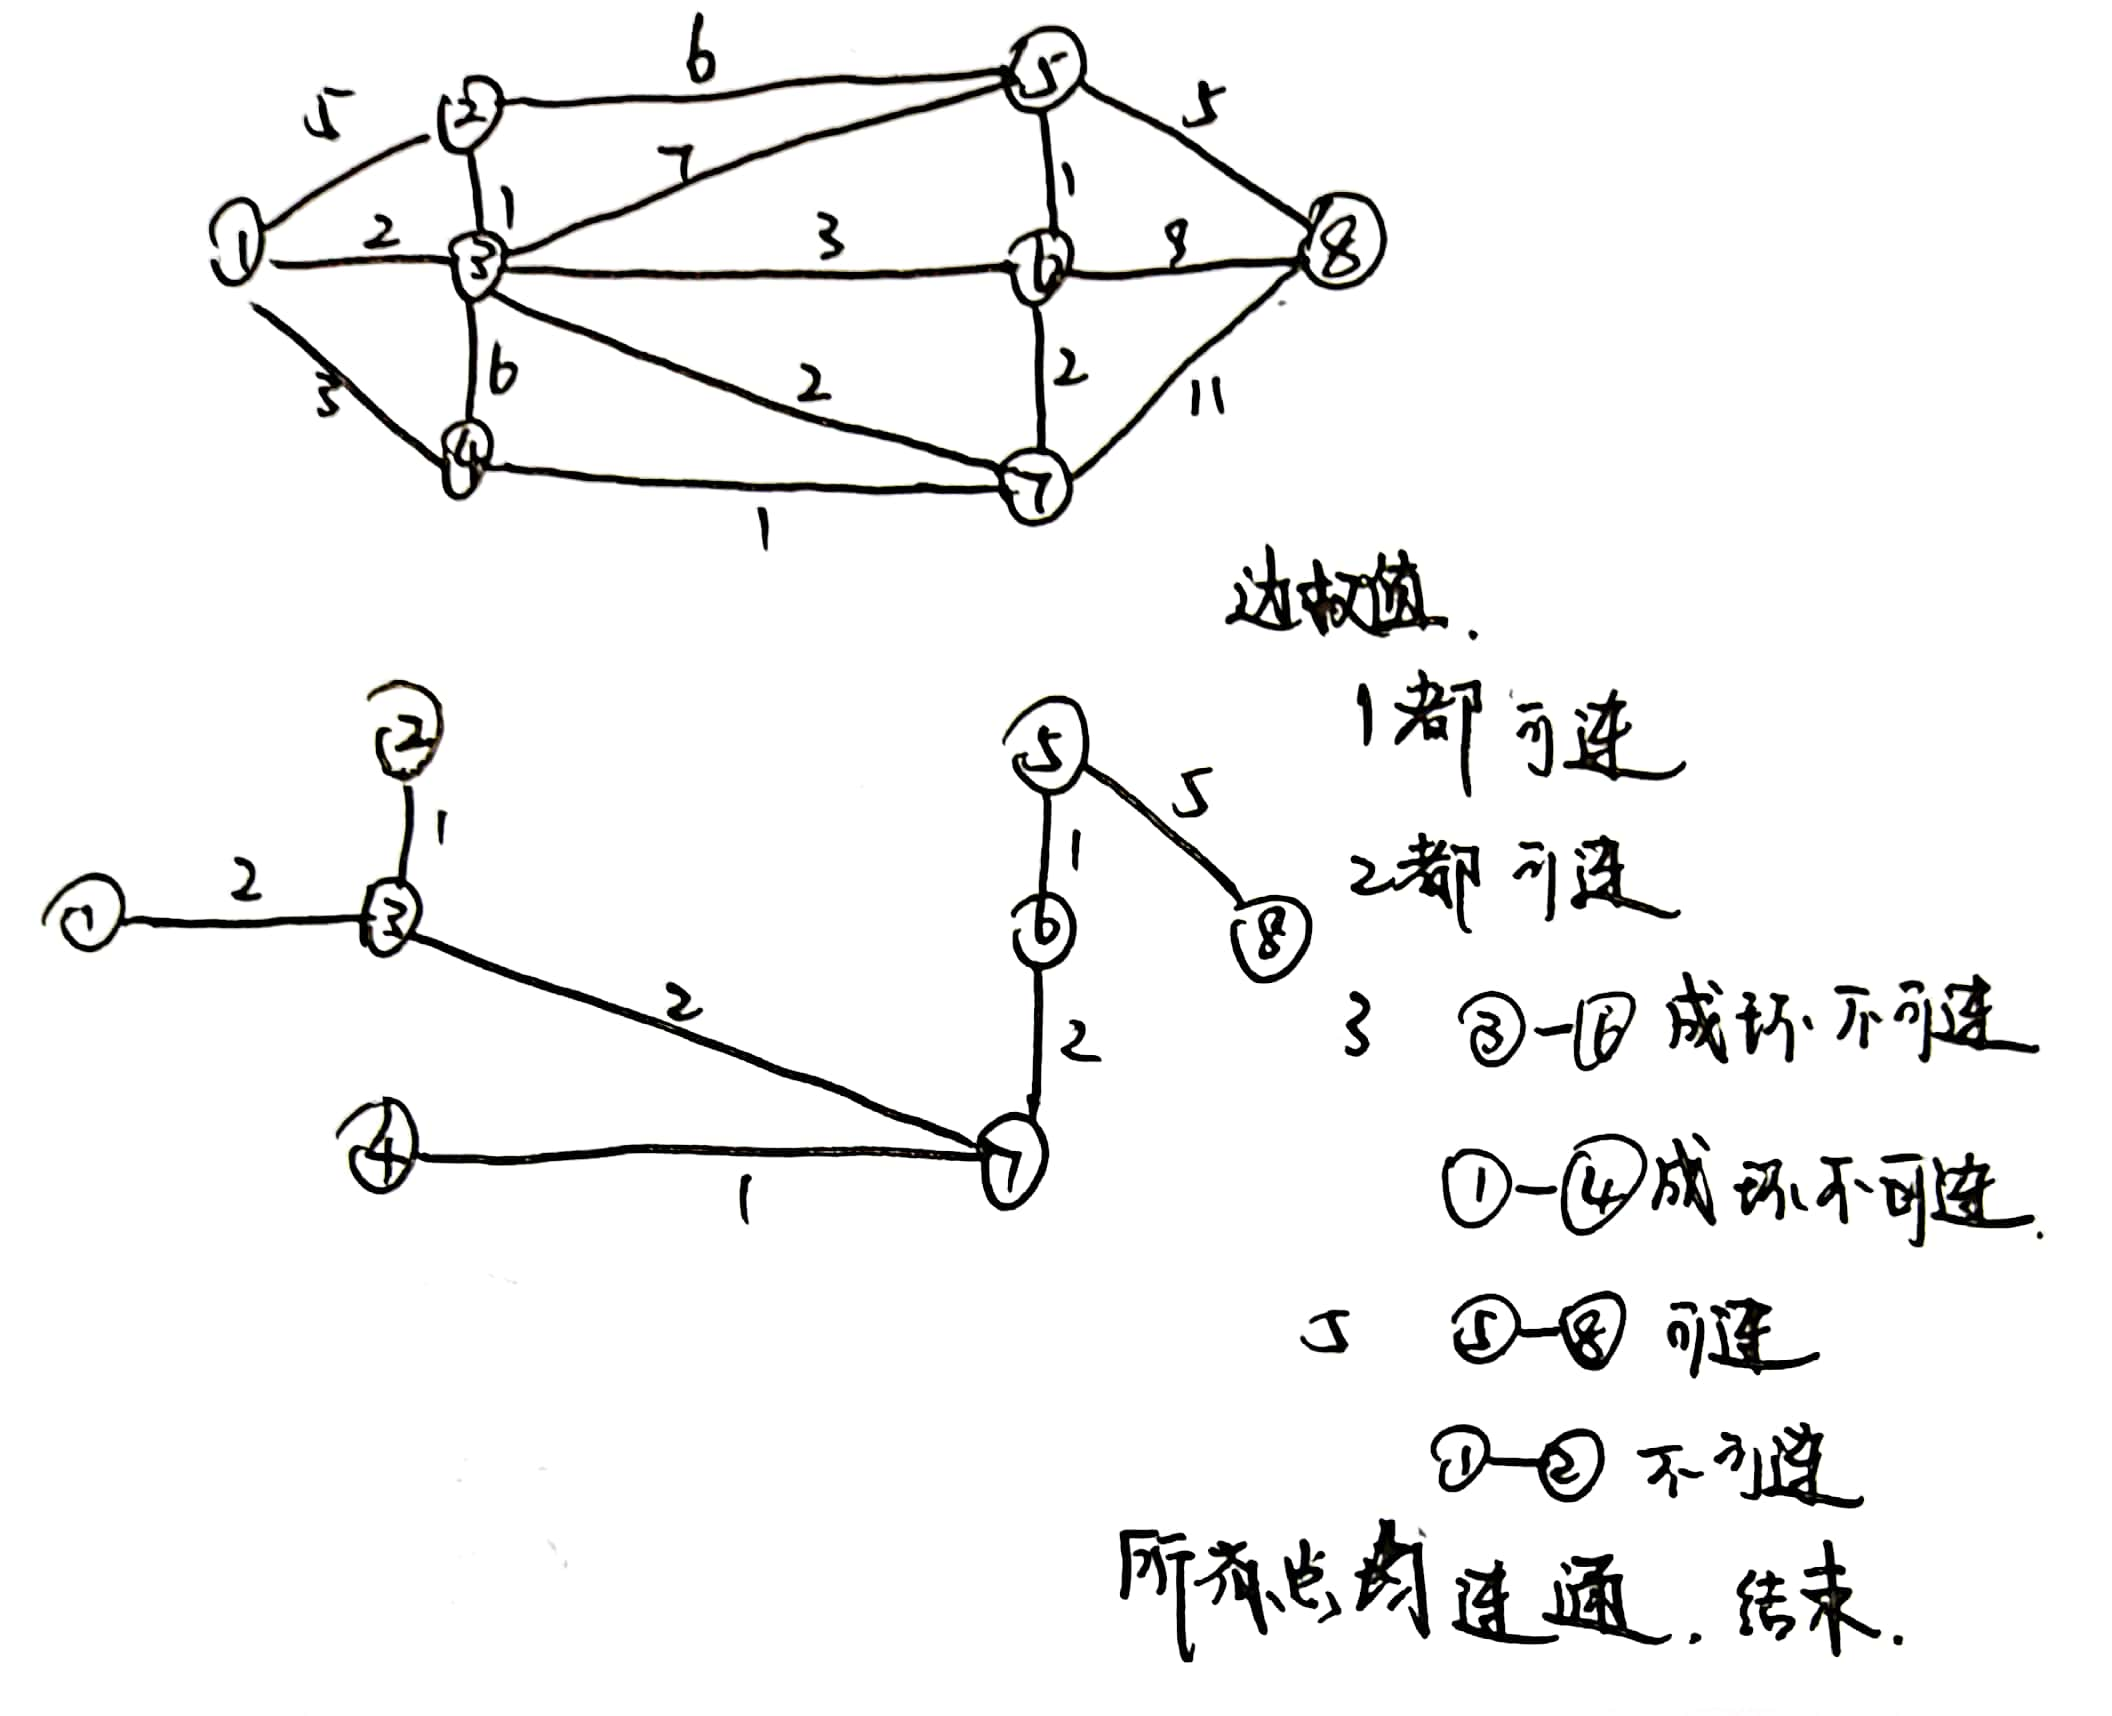
\includegraphics[width=0.8\textwidth]{graph.jpg}
    }
\end{solution}

\end{document}
